\documentclass[12pt, man]{apa6}
\usepackage[american]{babel}
\usepackage{csquotes}
\usepackage[style=apa,sortcites=true,sorting=nyt,backend=biber]{biblatex}
\usepackage{graphicx}
\DeclareLanguageMapping{american}{american-apa}
\addbibresource{ref.bib}


\abstract{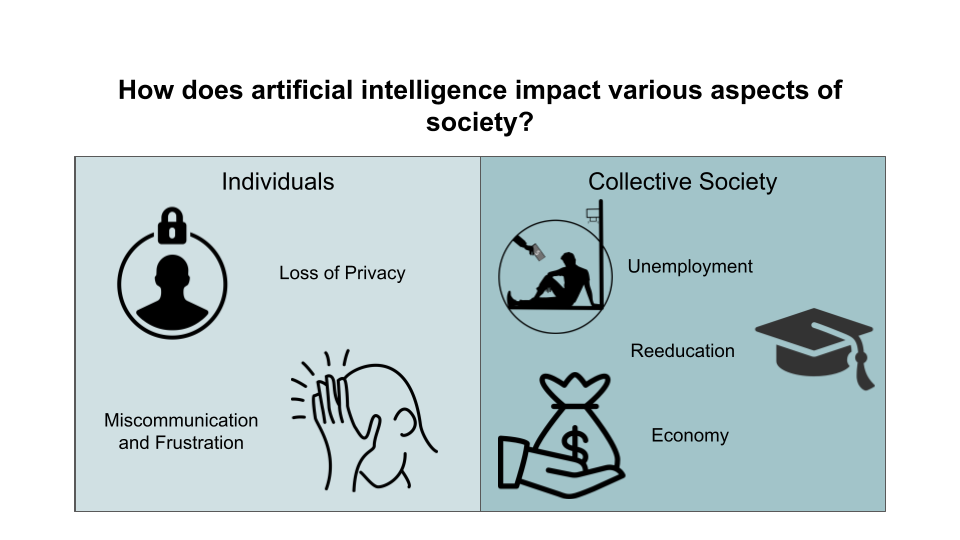
\includegraphics[width=\textwidth]{visualAbstract.png}}

\keywords{Artificial intelligence, automation, algorithms, data collection, economy, consumer, engagement, unemployment}

\title{The Impact of Artificial Intelligence on Society}
\shorttitle{AI and Society}

\author{Garrett Price}
\affiliation{Brigham Young University}

\rightheader{AI and Society}
\begin{document}
\maketitle

Artificial Intelligence has been misunderstood by the masses ever since the term was conceived.  Media has greatly exaggerated the potential
benefits and drawbacks to this AI revolution.  These misconceptions of what artificial intelligence is and can do lead to concern. Many people question
whether AI has a place in our world and do not fully understand the benefits. Others are eager to implement automation in many aspects but are unaware of the
potential drawbacks.  For the purposes of this article, artificial intelligence refers to any form of automation by technology, such as cleaning robots or algorithms used on social media sites to display certain posts.

This article seeks to address these concerns by combining the findings of studies from across the globe to clarify how AI can impact various aspects of life.  While the available research is extensive, it cannot provide a definitive answer of how AI will impact society due to the rapidly evolving nature of the field.  However, the results and conclusions from the current studies do provide enough information to see how AI has affected society up until now.  These effects can be changed according to how governments, tech firms, and employees react to the growing influence of AI.

This paper will address how AI has affected many aspects of life and what can be done to limit or increase the impact of AI.  Firstly, the changes in individual's lives will be discussed.  The areas discussed include the negative impact on personal privacy, changes to consumer interactions, the impact on employment, and the increased education needed to sustain one's current quality of life.  Later, the impact on the public as a whole will be analyzed.  AI can impact economies on a local or a global scale by decreasing or increasing unemployment rates in various sectors.  It also can be used to manipulate and control populations through misinformation and other strategies.

\section*{Impact of AI on Individuals}
Consumers are having more interactions with AI as businesses automate more aspects of the consumer experience.  Any situation in which a consumer interacts with an AI, knowingly or not, to achieve something can be considered when discussing AI's impact on consumers.\\
\subsection*{Personalized Experiences and Loss of Privacy}
The use of AI to collect and analyze data in consumer experiences leads to drastically different interactions with each consumer \parencite{Puntoni2021}.  These personalized experiences can make it easier for consumers to get what they want.  For example, one heavily personalized experience would be a social media feed.  The implemented algorithms collect data of the user and find similar posts that the user is likely to interact with.
This type of interaction with AI can be good for the consumer if it is what they expect.  Receiving recommendations based on interests can lead to a more fulfilling experience for the consumer.  It can also forge a relationship between the consumer and the company \parencite{Kumar2019}.  However, this application of AI can lead to users feeling vulnerable and exploited if not handled properly.  Aguirre et al. \parencite*{Aguirre2015} made the observation that "covert data collection", or the act of collecting data without the consumer's knowledge or consent, causes users to feel uncomfortable and can backfire on the company as the consumer stops interacting with them due to loss of trust.  Kumar and Aguirre have differing thoughts on the lasting impact this data collection can have on a consumer.  Kumar's claims of increased trust and a stronger relationship can be true, but Aguirre's study showing that covert data collection negatively impacts consumer's views of the company show that the wrong implementation of data collection will lead to the opposite of Kumar's claim.

Puntoni et al. \parencite*{Puntoni2021} claimed that as technology has become more central to life, consumers lose more ownership of their own personal data. This collection of data causes people to fear a "surveillance state" where everything they do and say is recorded.  This state has slowly become a reality as now words heard by speakers in the home to movies selected on Netflix are all fed to one company's AI or another to control what the user experiences next. As stated above, consumers are made uncomfortable by covert data collection.  It starts to become a trade-off for people as they weigh the benefits of a tailor-made experience and the cost of losing ownership of personal data.

What needs to be done to make these experiences better for the individual?  Aguirre's \parencite*{Aguirre2015} results have shown that personalization leads to more interaction by consumers companies are more transparent with how they collect the user's data while no change was noted when companies use more covert strategies.  For consumers to have a better experience with AI personalization companies must be up front with what data they are collecting and how it will be used.  There is currently no widely accepted standard of ethical use of AI in fields such as marketing \parencite{Puntoni2021}.  In order to protect consumers' privacy and personal data, there must be some sort of guideline for companies to follow on what is ethical or not.  Puntoni agrees with Aguirre's overall statement that personalization leads to better experiences for consumers, but recommends some sort of regulation to avoid situations like those that Kumar described.

\subsection*{Service AI and Consumers}
People want an AI to make certain tasks easier \parencite{Trivedi201991}.  For this section, chatbots, or AI that chat with users for purposes such as customer service, will be discussed.  They are a prime example of a service AI that attempts to make something easier for an individual and there has been much research on their effectiveness.  While only one example will be dissected, the same ideas to improve chatbot functionality can also be applied to other service AI.

Chatbots have many clear benefits for the consumer and for the business.  They allow for access to customer service at any hour, they are fast and efficient, and they are able to help more people than a human chat agent \parencite{McLean2017494}. These aspects make receiving customer support quick and easy for the consumer.  Trivedi \parencite*{Trivedi201991} observed that effective use of chatbots can also increase the trust consumers have in the company.  However, the "service quality, information quality, and system quality" customers experience impact their interactions more than any of the benefits above \parencite{McLean2017494}.  No customer will leave feeling satisfied with the service they received from the AI if the information given was incorrect, the responses were slow, or the interface was difficult to understand.  The ideas of service, information, and system quality are important for determining how to improve the customer's experience with the service AI.  These aspects are able to be observed easily through surveys directed to the consumer or tests under various circumstances.  These should be the first things that companies seek to improve if they want a better experience for their customers.

Wirtz \parencite*{Wirtz2018} observed in a study that robots that can "mimic the expression" of a person are perceived as more "pleasant" and customers are more willing to interact with them.  Mclean, Graeme, and Frimpong \parencite*{McLean2017494} observed a similar effect with their chatbot studies and the use of emoticons.  However, they do disagree about their importance.  Wirtz \parencite*[]{Wirtz2018} stated that the "warmth" of the service AI is as impactful as its ability.  Mclean \parencite*[]{McLean2017494} claimed that while emotion expressed through empathy and emoticons has a positive influence, it does not greatly impact the overall experience.  Trivedi \parencite*{Trivedi201991} agreed with Mclean in that the quality of the overall service and result is more important than the perceived personality of the AI.

\subsection*{Employment}
On the other end of the consumer interaction, individuals can be affected in their work.  Service robots and other forms of automation are becoming more prevalent. In the example above, the chatbots are replacing or working along side humans in their job as chat agents.  This integration of AI into the workforce has been a cause of concern due to the unknown impact on the human workers \parencite{DeCanio2016280}.

Firstly, the potential impact on the wages of the human employees will be discussed.  Decanio \parencite*[]{DeCanio2016280} noted that if human labor could easily be substituted with robot labor, then the wages paid to those humans would likely decrease as AI solutions are implemented in their field.  They did not observe a definitive number or percentage by which the wages would decline.  Frey and Osborne \parencite*[]{Frey2017} observed a similar negative relationship between worker wages and the probability of automation.

This spreading of AI does not mean that workers' quality of life will decline due to lesser wages.  As more jobs become automated, people will need to spend less money on those services.  Decanio \parencite*[]{DeCanio2016280} gave the example of a cleaning robot; The growing market of household robots can save people money as they will not need to hire housekeepers or caretakers for the elderly.  Frey and Osborne agree with Decanio in that worker's quality of life will not decrease drastically, but they explain it is due more to the inevitable change in employment that workers will need to obtain through obtaining more education.

\subsection*{Reskilling and Upskilling}
As AI replaces more workers in many industries \parencite{Nguyen2022}, these people will need to find new jobs.  Many of these jobs at risk of automation are described as "low-skill" and "low-wage" \parencite[]{Frey2017}.  Frey and Osborne \parencite*[]{Frey2017} also observed a "strong negative relationship" between the education required for a position and the probability that position could be performed by AI in the future.
There are currently many more low-skilled workers compared to medium-skilled and high-skilled employees.  Willcocks \parencite*[]{Willcocks2020} estimated that at the end of 2020 there would be a surplus of 95 million low-skilled workers and a deficit of 85 million medium-skilled and high-skilled workers.

For individuals to benefit, they will need to take the initiative and move ahead of the wave of AI.  Frey and Osborne \parencite*[]{Frey2017} believe that low-skill workers will begin to transition to jobs that are not as likely to be replaced by AI. The demand and availability for new and higher skills will increase \parencite{Willcocks2020}.  These are often jobs that require some creative or free-thinking capacity that cannot be easily performed by machines.  These jobs also tend to have higher wages \parencite{Frey2017}.  Willcocks and Frey agree that these higher skill jobs will be filled by the previously low-skilled workers as they seek new and higher education.

As people begin to gain new education and training, they will be able to fulfill the demand for these higher-paying roles.  Companies and developers of AI should seek AI solutions that make some tasks easier while still allowing human contribution through creativity, social skills, and other uniquely human aspects \parencite[]{Kolade2022}.  If both individuals and corporations follow this plan, the "AI revolution" can improve the standard of life for everyone \parencite{Makridakis2017}.  Kolade and Makridakis agree that life will be better overall for people as AI begins to do the tedious and physically-demanding jobs, allowing humans to do more creative and skillful jobs.  This leads to an increase in income for many and can help peiple feel more satisfied with their work, leading to more happiness \parencite{Makridakis2017}.

\section*{Impact of AI on society}
The second part of this paper will focus on how the growing influence of artificial intelligence has impacted the society as a whole.  Many of the changes impacting individuals will be compounded on a larger scale and end up having a greater impact on the world around them.

\subsection*{Economic Impact}
As discussed previously, AI has begun to threaten human jobs, especially in lower-skilled fields \parencite{Huang2018}.  This replacement will increase unemployment rates.  Nguyen and Vo \parencite*{Nguyen2022} observed that unemployment rates will continue to rise with the rate of AI replacement until an inflation threshold is met.  They noted that "developing markets, especially those with considerable inflation levels," would be able to take advantage of this pattern and implement AI solutions more aggressively compared to developed nations as their unemployment rate will not be negatively effected due to their higher inflation rate.  Provided these developing nations can control their inflation, they will benefit from adopting AI replacement strategies.

Developing markets can also be influenced by the AI solutions implemented in established economies.  A study by Gravina and Pappalardo \parencite*{Gravina2022} observed that differences in automation levels in developed European countries strongly correlated to changes in unemployment rates in budding markets.  The impact varies by field and by geography.  They noted that in industries that are more susceptible to automation, the negative effect on the unemployment rate would be nearly double compared to the effect in less at-risk sectors.  However, automation in fields of "non-tradeable" services appeared to create local jobs to accompany the automation. Gravina and Pappalardo also determined that Asian countries were impacted up to three times more than South American countries by European robotization.  Kaplan and Haenlein \parencite*{Kaplan2020} call upon the leaders of the world to take actions to assure that the use of AI in their countries and markets do not negatively impact other economies by putting regulations and guidelines into place to limit the drawbacks.  Kaplan and Gravina both recognize that without regulation, AI replacement poses a threat to emerging economies and agree that the best way to minimize the impact is to limit AI solutions to local non-tradeable sectors.

\subsection*{Social Impact}
Kaplan and Haenlein \parencite*{Kaplan2020} warn not only about the economic dangers of misuse of AI but also of the social problems that can be amplified as more aspects of life become automated.  As AI becomes more integrated into society, it does not affect everyone equally.  They warn that AI can widen the economic inequality gap due to an increase in worker productivity and a decrease in money spent by firms on wages.  They claim this "rise in inequality is the greatest societal concern" of the AI revolution.  As the leaders of these tech companies accrue more wealth, social and political tensions begin to develop \parencite{Arogyaswamy2020}.

The wealth inequality is only the beginning of the power tech leaders can obtain thanks to AI.  As discussed earlier, data collection serves as a key part to many of the AI systems people interact with on a daily basis.  Firms such as Facebook and Google collect countless amounts of data from their users and can use it to their gain \parencite{Arogyaswamy2020}.  Arogyaswamy \parencite*{Arogyaswamy2020} observed that social media algorithms have been designed to be addictive and captivate the attention of users.  They encourage "narcissistic" behaviors and isolate people from those around them.  The AI controlling the next post on a user's feed will try to pick the most engaging post, and often times this manipulation may have adverse effects.  Arogyaswamy \parencite*{Arogyaswamy2020} noted that hate speech and other harmful content will be spread quickly by these algorithms due to the strong reactions they incite.  Misinformation and rumors reach millions of people without any regulation or restriction.  These AI can be weaponized by people in power, such as governments or even the leaders of the tech firms themselves.

These platforms cannot be held responsible for the content users upload to them \parencite{Arogyaswamy2020}, but some form of regulation will be necessary sooner or later.  Regulation requires more research, especially as it could have the most drastic impact on the public.

\section{Conclusion}
Key points include AI makes people get more education to have jobs, it creates jobs while also taking them away from people, it can increase societal pressures through misinformation and inequality.  Further research should be done on the impact it can have on higher skilled jobs, effective regulations for implementation of AI, impacts on other areas such as education and home life.








\printbibliography

\end{document}